%%%%%%%%%%%%%%%%
% Metodolog\'ia, An\'alisis y Dise\~no
%%%%%%%%%%%%%%%%


\section{Metodolog\'ia}

\subsection{Metodolog\'ia en cascada}

\noindent Para este proyecto, se decidi\'o utilizar la metodolog\'ia de \textbf{desarrollo en cascada},  la cual es una metodolog\'ia de gesti\'on de proyectos que organiza el trabajo en fases secuenciales, donde cada etapa debe completarse antes de iniciar la siguiente\cite{asanaQueEsMetodologia}. Se eligi\'o esta metodolog\'ia debido a que se requer\'ia definir los requisitos con exactitud desde el inicio del proyecto, adem\'as de que debido a la dificultad para reuniones constantes con el equipo del proyecto Foodprice, no era adecuado el uso de una metodolog\'ia \'agil. 


\begin{figure}[H]
    \centering
    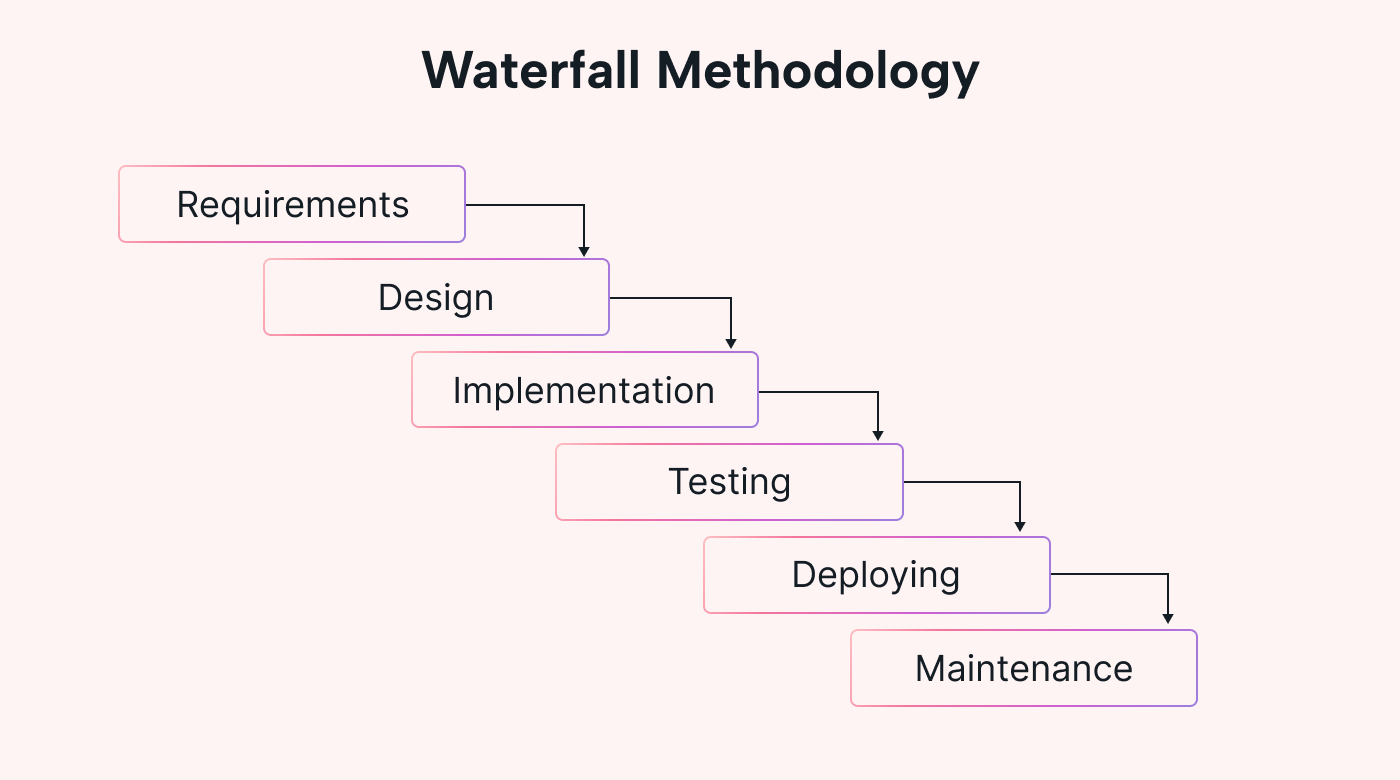
\includegraphics[width=15cm]{img/metodologia/metodologia waterfall.png}
    \caption{Metodolog\'ia en Cascada en el Desarrollo de Sistemas}
    \label{fig:metodologia_waterfall}
\end{figure}


\noindent Las etapas de desarrollo en esta metodolog\'ia son como se ve en la Figura \ref{fig:metodologia_waterfall} consisten en:

\begin{enumerate}
    \item \textbf{Requerimientos:} Esta fase consiste en recolectar toda la informaci\'on posible para garantizar el \'exito del proyecto. Aqu\'i se identifican las funcionalidades necesarias, las especificaciones t\'ecnicas y las expectativas del cliente. Es la fase m\'as esencial de la metodolog\'ia en cascada, ya que al no retroceder a pasos anteriores, se requiere definir cada detalle lo mejor posible desde el principio para evitar errores en pasos posteriores.

    \item \textbf{Dise\~no: } En esta fase se dise\~{n}a c\'omo funcionar\'a el sistema a nivel t\'ecnico. Se eligen las tecnolog\'ias y herramientas que se utilizar\'an. Y se crean diagramas como los siguientes:

    \begin{itemize}
        \item Dise\~no UML de la arquitectura del sistema
        \item Modelado de datos
        \item Diagramas de caso de uso
    \end{itemize}
    \item \textbf{Implementaci\'on: } Una vez que el dise\~{n}o est\'a completo, se comienza a desarrollar el software siguiendo las especificaciones. Esta fase se centra en la codificaci\'on de las funciones definidas en las etapas anteriores.

    \item \textbf{Pruebas: } Esta etapa tiene como objetivo verificar que el sistema funciona correctamente y cumple con los requisitos. Por lo cual en esta etapa el software es sometido a diversas pruebas para garantizar su correctitud. Entre las pruebas m\'as comunes se encuentran las pruebas unitarias (de cada componente), pruebas de integraci\'on (c\'omo funcionan los componentes juntos) y pruebas de aceptaci\'on (ver si el sistema cumple con los requisitos del cliente).

    \item \textbf{Despliegue: } En esta fase, despu\'es de que el sistema pas\'o todas las pruebas, se procede a desplegar el software en el entorno donde ser\'a utilizado. Y pueden empezar a interactuar los usuarios con el sistema directamente.

    \item \textbf{Mantenimiento:}  Despu\'es del despliegue, solo queda la fase de mantenimiento, la cual consiste en asegurar el correcto funcionamiento del sistema en un plazo de tiempo, as\'i como realizar las mejoras y correcciones necesarias.

    
\end{enumerate}



\subsection{Tipo de Estudio}

\noindent Con base en la finalidad de este proyecto, la cual es mejorar la calidad de vida de las personas de escasos recursos al ofrecerlos  una herramienta que les provea con una dieta que se adapte a sus necesidades nutricionales y econ\'omicas; este proyecto se categoriza como un \textbf{estudio aplicado de desarrollo tecnol\'ogico, con un enfoque mixto (cualitativo - cuantitativo)}.
\\
\\
Esta clasificaci\'on se alinea con las caracter\'isticas del proyecto, siendo un estudio aplicado de desarrollo tecnol\'ogico ya que busca principalmente utilizar la tecnolog\'ia como un medio para crear una soluci\'on pr\'actica y funcional que impacte positivamente la vida de sus usuarios. Y cuenta con un enfoque mixto (cualitativo - cuantitativo), ya que el impacto que genere no se medir\'a solo de manera num\'erica, sino haciendo uso tambi\'en de m\'etodos cualitativos como encuestas sobre la percepci\'on del software y su utilidad; para as\'i proporcionar no solo resultados medibles y replicables, sino que tambi\'en contextualiza el impacto real de la soluci\'on en la vida de los usuarios.

\section{Requerimientos}
\noindent En el desarrollo de este proyecto, la fase de An\'alisis de requerimientos es el paso m\'as esencial del proceso de desarrollo, debido a las razones mencionadas anteriormente de las caracter\'isticas de la metodolog\'ia en cascada. Por esto, se requiri\'o de investigar y analizar de forma exhaustiva el panorama de los sistemas de generaci\'on de dietas, para entender c\'omo lograr un impacto en este campo, y alcanzar especialmente a la poblaci\'on objetivo, siendo estas personas en condici\'on de pobreza o vulnerables econ\'omicamente. 
\\
\\
A su vez, para la expansi\'on del proyecto Foodprice, un factor clave es la obtenci\'on de precios que reflejen la realidad de lo que encontrar\'a la persona promedio en los estantes de un supermercado.
\\
\\
Adem\'as de esto, otro aspecto clave del proyecto es el encontrar la mejor manera de trabajar con la aplicaci\'on en R de Foodprice, para poder utilizarla en una aplicaci\'on web de forma m\'as sencilla y \'optima, expandiendo el proyecto Foodprice, facilitando as\'i la posibilidad de que llegue a ser usada con m\'as frecuencia en otros proyectos.
\\
\\
Teniendo estos puntos en cuenta, se presenta la necesidad tambi\'en de entender cuales son las mejores maneras de que una aplicaci\'on web sea funcional para la mayor variedad de dispositivos,  y accesible para personas independiente de su nivel de experticia con la tecnolog\'ia.
\\
\\
Para poder lograr una fase de an\'alisis de requerimientos exitosa, se decidi\'o comenzar por definir requerimientos de investigaci\'on, funcionales, y no funcionales. Despu\'es de esto, se proceder\'a al desarrollo de los requerimientos de investigaci\'on, la definici\'on del arquetipo de usuario (poblaci\'on objetivo), y diagrama de casos de uso. Despu\'es de esto se estudiar\'a la decisi\'on de las herramientas que se usar\'an, junto con sus ventajas y desventajas. Y con esto se proceder\'a a continuar con la fase de dise\~{n}o teniendo unas bases s\'olidas para un proyecto bien estructurado.


\subsection{Levantamiento de Requerimientos}

\noindent Es preciso que se aclare que los temas de investigaci\'on a pesar de que se plantearon en el proyecto, no forman parte de los requerimientos de un desarrollo de software por ello se manejan como un tipo de requerimiento distinto a los usuales: Funcional y No funcionales.
\\
\\
\noindent Como Requerimientos Funcionales se entiende  que son todos aquellos requerimientos que el usuario final exige espec\'ificamente como prestaciones b\'asicas que debe ofrecer el sistema. Todas estas funcionalidades deben estar necesariamente incorporadas al sistema como parte del contrato. Estos se representan o establecen en forma de entrada que se le dar\'a al sistema, la operaci\'on realizada y la salida esperada. Son b\'asicamente los requisitos declarados por el usuario que se pueden ver directamente en el producto final, a diferencia de los requisitos no funcionales\cite{geeksforgeeks_2020}.
\\
\\
\noindent Como Requerimientos no funcionales se entiende que son todos aquellos requerimientos que tienen que ver con la calidad, son b\'asicamente las restricciones de calidad que el sistema debe satisfacer seg\'un el contrato del proyecto. La prioridad o la medida en que se implementan estos factores var\'ia de un proyecto a otro. Tambi\'en se les llama requisitos no conductuales\cite{geeksforgeeks_2020}.

\subsection{Requerimientos de investigaci\'on}

\begin{longtable}[c]{| p{.20\textwidth}  | p{.40\textwidth}  | p{.30\textwidth}  |}
    \caption{Tabla requerimientos de investigaci\'on}
    \label{tab:Tabla requerimientos de investigacion}
         \\ \hline \textbf{RI\# - T\'itulo} & \textbf{Descripci\'on} & \textbf{Criterio de aceptaci\'on}  \\ \hline
         \textbf{RI01 -- Caracter\'isticas de sistemas de generaci\'on de dietas} & \begin{itemize}
             \item Se debe lograr entender cuales son las caracter\'isticas principales de los sistemas de generaci\'on de dietas que existen en la actualidad.
             \item Observar que opciones permiten estos sistemas, y que limitantes tienen
         \end{itemize} & \begin{itemize}
             \item Se investiga sobre software que haga un trabajo relacionado, idealmente que genere dietas.
             \item Se enumeran caracter\'isticas que sean clave para la generaci\'on de dietas en estos software.
             \item Se determina que caracter\'isticas y opciones tendr\'a el software de este proyecto.
         \end{itemize} \\\hline
         
         \textbf{RI02 -- Mejor m\'etodo de obtenci\'on de datos con impacto real} & \begin{itemize}
             \item Se estudia que supermercados reflejan mejor la realidad del consumidor promedio, y por qu\'e motivos.
             \item Se determina que supermercado es pertinente para este proyecto.
             \item Se explican las razones del por qu\'e se elije este.
             \item Se analiza de que maneras se pueden obtener los datos que reflejen  los precios reales.
         \end{itemize}& \begin{itemize}
             \item Se comparan de forma eficaz los supermercados con mayor impacto de colombia.
             \item se proveen razones l\'ogicas que soporten la decisi\'on del mercado que se usar\'a para este proyecto.
             \item Se establece como se obtendr\'an los datos de dicho supermercado.
         \end{itemize} \\  \hline
        
\end{longtable}


\subsection{Requerimientos Funcionales}

\begin{longtable}[c]{| p{.20\textwidth}  | p{.40\textwidth}  | p{.30\textwidth}  |}
    \caption{Tabla requerimientos funcionales}
    \label{tab:Tabla requerimientos  funcionales}
         \\ \hline \textbf{RF\# - T\'itulo} & \textbf{Descripci\'on} & \textbf{Criterio de aceptaci\'on}  \\ \hline
         \textbf{RF01 -- Generaci\'on de las dietas} & \begin{itemize}
             \item El sistema debe permitir al usuario generar una dieta diaria que cubra sus necesidades nutricionales b\'asicas al menor costo posible, basado en la informaci\'on de precios de alimentos.
         \end{itemize} & \begin{itemize}
             \item La dieta generada debe cubrir al menos el 100\% de los requerimientos diarios de calorías.
             \item La dieta generada debe ser de costo m\'inimo.
             \item La dieta generada debe tomar en cuenta las caracter\'isticas que el usuario elija, as\'i como las restricciones.
             \item La dieta debe indicar el valor cal\'orico o nutricional diario que suple, as\'i como el costo total de comprarla en el mercado del que se obtenga la informaci\'on
             \item Cada alimento que hace parte de la dieta, debe ir acompa\~{n}ado de una imagen, precio, informaci\'on nutricional, y link sobre donde pueden encontrar el producto.
         \end{itemize} \\\hline
         
         \textbf{RF02 -- Visualizaci\'on de las dietas} & \begin{itemize}
             \item Se debe poder visualizar de forma sencilla y clara la dieta que genere el sistema.
         \end{itemize}& \begin{itemize}
             \item El sistema debe mostrar de una forma clara la dieta generada para dicho usuario en base a las caracter\'isticas que este defini\'o.
         \end{itemize} \\  \hline


         \textbf{RF03 -- Selecci\'on del tipo de dieta} & \begin{itemize}
             \item El sistema debe permitir elegir entre 3 tipos de dietas, las cuales pueden suplir necesidades cal\'oricas (cubre la cantidad de calor\'ias necesarias para el funcionamiento del cuerpo), nutricionales (cubre la cantidad de calorias y nutrientes para el funcionamiento del cuerpo), o ser una dieta recomendada o saludable, y variada.
         \end{itemize}& \begin{itemize}
             \item El sistema debe permitir al usuario seleccionar cual de estas 3 dietas prefiere generar.
             \item El sistema debe adaptarse a la dieta generada, y generar la correspondiente.
         \end{itemize} \\  \hline

         \textbf{RF04 -- Selecci\'on de caracter\'isticas del usuario} & \begin{itemize}
             \item El sistema debe permitir seleccionar una serie de caracte\'isticas, las cuales tienen un impacto en el tipo de dieta necesaria, y adecuar la dieta a estas.
         \end{itemize}& \begin{itemize}
             \item El sistema debe contar con una lista de caracter\'isticas f\'isicas, las cuales tengan un impacto en la dieta que se genere.
             \item El sistema debe tener en cuenta estas caracter\'isticas a la hora de generar la dieta para el usuario.
         \end{itemize} \\  \hline

          \textbf{RF05 -- Selecci\'on de restricciones} & \begin{itemize}
             \item El sistema debe permitir seleccionar una serie de alimentos los cuales no desea que hagan parte de la dieta, y estos deben ser tomados en cuenta y no hacer parte de la dieta final, siendo reemplazados por otros alimentos.
         \end{itemize}& \begin{itemize}
             \item El sistema debe contar con una lista de alimentos, los cuales pueda seleccionar el usuario para indicar que no desea que hagan parte de su dieta.
             \item Debe permitir seleccionar varios alimentos, y todos tenerlos en cuenta.
             \item La dieta generada no debe tener ninguno de los alimentos que se restringieron.
         \end{itemize} \\  \hline

         \textbf{RF06 -- Nombre del usuario de la dieta} & \begin{itemize}
             \item El sistema debe permitir al usuario ingresar su nombre, y este dato debe verse reflejado en su dieta, esto para permitir con mayor facilidad al usuario saber que esa dieta en espec\'ifico le pertenece.
         \end{itemize}& \begin{itemize}
             \item El sistema debe contar con un campo en el que el usuario pueda escribir su nombre.
             \item El nombre del usuario debe verse en la dieta y en el archivo PDF asociado a esta.
         \end{itemize} \\  \hline

\end{longtable}


\subsection{Requerimientos No Funcionales}


\begin{longtable}[c]{| p{.20\textwidth}  | p{.40\textwidth}  | p{.30\textwidth}  |}
    \caption{Tabla requerimientos no funcionales}
    \label{tab:Tabla requerimientos no funcionales}
         \\ \hline \textbf{RNF\# - T\'itulo} & \textbf{Descripci\'on} & \textbf{Criterio de aceptaci\'on}  \\ \hline
         \textbf{RNF01 -- Accesibilidad de la p\'agina - colores} & \begin{itemize}
             \item El sistema debe cumplir con los est\'andares de accesibilidad respecto a contrastes de colores definidos en la Web Content Accessibility Guidelines (WCAG)
         \end{itemize} & \begin{itemize}
             \item El contraste entre el fondo y los textos debe tener un ratio de contraste de 4.5:1 para texto normal (peque\~{n}o), y 3:1 para texto grande (18 pt o m\'as).        
         \end{itemize} \\\hline
         
         \textbf{RNF02 -- Tiempos de carga razonables} & \begin{itemize}
             \item Se debe asegurar que los tiempos de carga al usar la herramienta sean razonables. Sobre todo al ir enfocado su uso a una poblaci\'on que podr\'ia no tener un internet tan veloz.
         \end{itemize}& \begin{itemize}
             \item El sistema no debe tardar m\'as de 3 segundos en la carga inicial de la p\'agina.
             \item El sistema no debe tardar m\'as de 5 segundos en la carga del plan de dieta, y la creaci\'on del PDF.
             \item Debe haber un tipo de indicador de que la p\'agina se encuentra cargando, para as\'i no haya problema aunque la carga tome m\'as tiempo por factores externos.
         \end{itemize} \\  \hline

         \textbf{RNF03 -- No hay errores con la combinaci\'on de caracter\'isticas y restricciones} & \begin{itemize}
             \item Se debe poder asegurar que sin importar que caracte\'isticas y restricciones se mezclen en la aplicaci\'on, esta siga funcionando con normalidad.
         \end{itemize}& \begin{itemize}
             \item Asegurar que ninguna mezcla de caracter\'isticas y restricciones genera un error en el sistema.
             \item Asegurar que se genere al menos una dieta de costo m\'inimo sin importar la mezcla de caracter\'isticas y restricciones que se tenga.
         \end{itemize} \\  \hline

         \textbf{RNF04 -- No permitir que se restrinjan todos los alimentos} & \begin{itemize}
             \item Debido a que no se puede generar una dieta sin alimentos, es necesario asegurar que el sistema no permita que el usuario restrinja todos los alimentos.
         \end{itemize}& \begin{itemize}
             \item El sistema debe indicarle al usuario que debe seleccionar al menos un alimento.
             \item El sistema no debe permitir que el usuario restrinja todos los alimentos.
         \end{itemize} \\  \hline

         \textbf{RNF05 -- El archivo PDF debe contener la dieta correspondiente} & \begin{itemize}
             \item La dieta que se exporte al archivo PDF para el usuario, debe contener los elementos principales de la misma dieta que genere el sistema para las caracter\'isticas y restricciones del usuario
         \end{itemize}& \begin{itemize}
             \item El sistema debe entregar los mismos alimentos y cantidades tanto para la aplicaci\'on web como para el archivo PDF en caso de la entrada ser la misma.
         \end{itemize} \\  \hline

        \textbf{RNF06 -- Si los par\'ametros de entrada permanecen constantes, la dieta generada debe ser consistente y presentar los mismos resultados} & \begin{itemize}
             \item Si los par\'ametros de caracter\'isticas y restricciones son iguales, el sistema deber\'ia arrojar la misma dieta, esto mientras no se hayan presentado cambios en la base de datos de alimentos.
         \end{itemize}& \begin{itemize}
             \item En el caso de generar una dieta en diferentes ocasiones, con las mismas entradas en caracter\'isticas y en restricciones, debe en todos los intentos generar la misma dieta. Mientras la base de datos no haya cambiado.
         \end{itemize} \\  \hline

         \textbf{RNF07 -- Conectar el paquete Foodprice a trav\'es de Python a la aplicaci\'on web} & \begin{itemize}
             \item El sistema debe funcionar en una constante comunicaci\'on entre R y Python, donde el middleware en Python se encargue de pasarle la informaci\'on al paquete Foodprice que necesita, y el paquete entregue la dieta de costo m\'inimo relacionada con la informaci\'on ingresada.
         \end{itemize}& \begin{itemize}
             \item El sistema debe ser capaz de comunicarse con el paquete de R de alguna forma a trav\'es de Python
             \item El sistema no deber\'ia interactuar con el sistema de R de forma directa sin Python.
             \item La conexi\'on entre R y Python debe garantizar el correcto funcionamiento del proyecto,
             
         \end{itemize} \\  \hline

         \textbf{RNF08 -- Testear la aplicaci\'on web con usuarios} & \begin{itemize}
             \item El sistema debe ser probado y funcionar adecuadamente con usuarios.
         \end{itemize}& \begin{itemize}
             \item El sistema debe ser probado con usuarios antes de su despliegue final.
             \item El sistema debe pasar dichas pruebas para considerarse que est\'a en un estado aceptable.
             \item Se deben documentar las opciones de mejora que los usuarios sugieran para trabajos futuros.
             
         \end{itemize} \\  \hline

\end{longtable}


\subsection{Desarrollo de requerimientos de investigaci\'on}
Con base en los requerimientos de investigaci\'on que se definieron anteriormente, se proceder\'a a su desarrollo, para cumplir con sus criterios de aceptaci\'on.

\subsubsection{RI01 -- Caracter\'isticas de sistemas de generaci\'on de dietas}

\noindent Para poder realizar de forma satisfatoria este proyecto, es necesario entender las bases que existen en la actualidad respecto a sistemas que cumplan un rol similar. Adem\'as de aquellos que se observaron en la secci\'on \ref{trabajosRelacionados}, podemos encontrar otros sistemas como lo son una herramienta del proyecto PlaSA Colombia, el cual se define como un ``espacio de f\'acil acceso en el que cualquier persona interesada en el universo del sistema alimentario encontrar\'a desde datos hasta narrativas a partir de informaci\'on veraz, sencilla y actualizada'' \cite{Nosotros}; este proyecto cuenta con una herramienta que muestra tres opciones de dieta, una saludable, una nutritiva, y una de subsistencia; y muestra el precio y los alimentos en los que se encuentra distribuida una dieta de costo m\'inimo para estos tipos de dietas. Adem\'as de esto, cuenta con una gr\'afica que muestra el costo diario de la dieta para diferentes grupos de edades, tanto para hombres como para mujeres.


\begin{figure}[H]
    \centering
    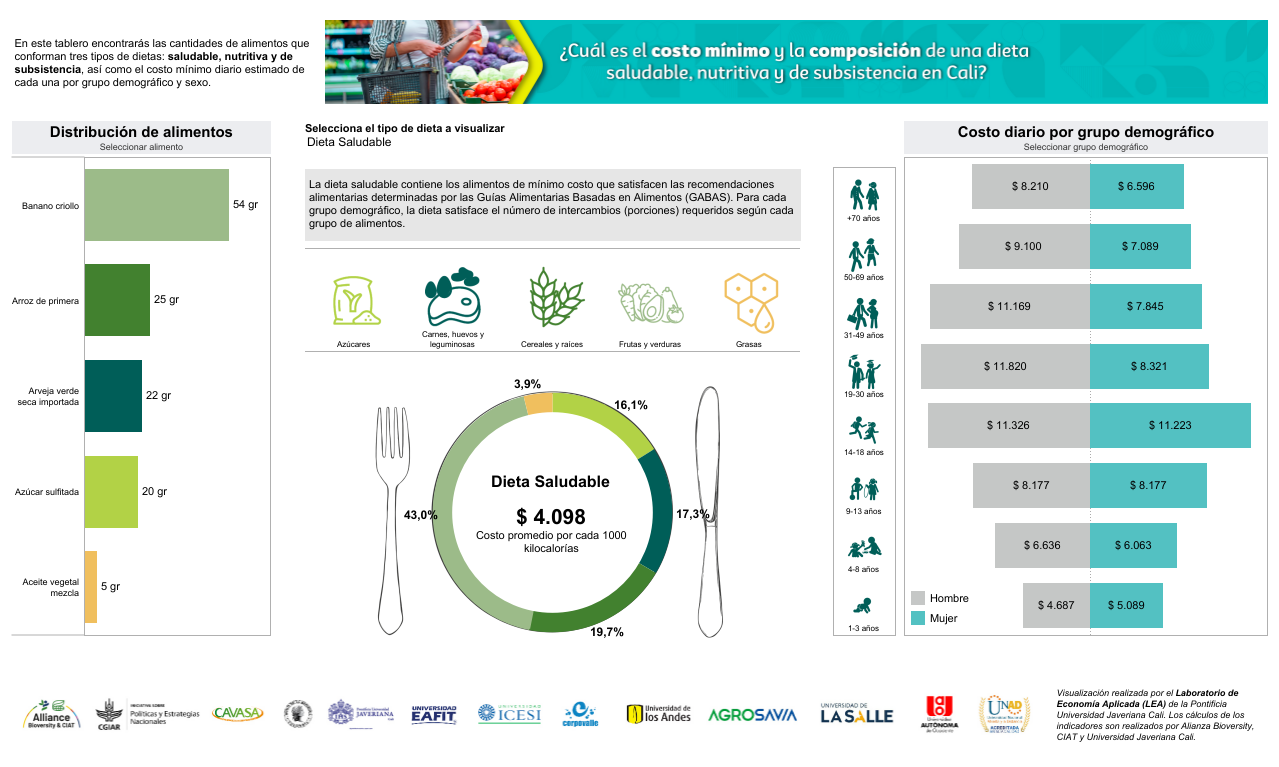
\includegraphics[width=15cm]{img/metodologia/Dashboard 1.png}
    \caption{?`Cu\'al es el costo m\'inimo y la composici\'on de una dieta saludable, nutritiva y de subsistencia en Cali?}
    \label{fig:plasaColombia}
\end{figure}

Este proyecto, como se puede observar en la figura \ref{fig:plasaColombia}, presenta informaci\'on \'util, de una forma organizada, sin embargo, presenta algunos problemas.

\begin{itemize}
    \item La base de datos de la que sacan los precios de sus alimentos, se encuentra bastante desactualizada, siendo esta del 2022.
    \item La base de datos toma los precios del Sistema de Informaci\'on de Precios y Abastecimiento del Sector Agropecuario (SIPSA) , por lo que estos no reflejan los precios con los que se encontrar\'a el consumidor final en las estanter\'ias.
    \item No funciona de forma correcta la opci\'on de seleccionar alguno de los Costo diario por grupo demogr\'afico; al seleccionar alguno el precio cambia, pero no refleja los datos que deber\'ia en la grafica de distribuci\'on de alimentos o en la gr\'afica central.
    \item No toma en cuenta la posibilidad de que una persona no pueda o no desee consumir un alimento en particular, por lo que puede que la dieta que provea no sea \'util para el usuario
\end{itemize}

A pesar de estos problemas, el acercamiento de PlaSA Colombia al reto que presenta crear un sistema as\'i es un gran avance, aportando en el panorama de herramientas \'utiles para disminuir los problemas de nutrici\'on en las poblaciones economicamente vulnerables. Se destaca que cuenta con caracter\'isticas como:

\begin{itemize}
    \item Gr\'aficas que muestran de forma visual los datos.
    \item Gr\'afica de la distribuci\'on de cada alimento en el total de la dieta diaria.
    \item Costo para dietas de diferentes grupos de edades y sexo.
    \item Una interfaz organizada y llamativa, con colores que ayudan a visualizar y diferencias los diferentes componentes de la dieta
\end{itemize}

Otro ejemplo de un sistema de generaci\'on de dietas, aunque con un enfoque mucho m\'as general y comercial, ser\'ia Diet Creator, el cual es un software para uso de nutricionistas, que les ayuda a crear dietas de forma r\'apida y sencilla para los usuarios de dichos nutricionistas, as\'i como les ayuda a llevar un control de los datos, para de esta forma tener un mejor control del avance y el manejo de dichas dietas.
\\
\\
Diet Creator, a pesar de no tratar un tema totalmente alineado con este proyecto, cuenta con algunas caracter\'isticas de las que se puede aprender, as\'i como un entendimiento de las dificultades y la importancia de utilizar una base de datos actualizada en un sistema como este, tal como se evidencia en la cita ``Todo software de nutrici\'on debe tener una base de datos de alimentos de fuentes cient\'ificas actualizadas, tambi\'en deber\'ia incorporar los productos reales del mercado, pero esto entra\~{n}a dificultades debido a que los productos son tan cambiantes que armonizar la informaci\'on es todo un reto global.''\cite{CongresoMundialNutricion}.
\\
\\
Este sistema es mucho m\'as comercial, ya que no es gratuito, y uno de sus principales puntos de venta es ayudar a nutricionistas en su trabajo. Sin embargo, es un software muy completo, que cuenta con una aplicaci\'on  muy intuitiva y con muchas herramientas, pero para lo relacionado con este proyecto, se pueden mencionar las siguientes caracter\'isticas:

\begin{itemize}
    \item Permite generar dietas personalizadas, con diferentes prop\'ositos.
    \item Permite seleccionar alimentos que no se quieran incluir en la dieta.
    \item Toma en cuenta muchos datos sobre el usuario, para que la dieta se adapte lo mejor posible a este.
    \item Provee toda la informaci\'on de una tabla nutricional para cada producto
    \item Entrega la informaci\'on de forma sencilla y profesional
    \item Permite descargar la informaci\'on para su impresi\'on o uso en general.
\end{itemize}

Sin embardo, a pesar de lo \'util que es esta herramienta, no cubre todas las necesidades que requiere este proyecto, al no incluir cosas como:

\begin{itemize}
    \item Precios para los alimentos
    \item Opci\'on de dieta de costo m\'inimo
\end{itemize}

Con lo observado en estos sistemas, se eligen entonces como caracte\'isticas clave para el sistema de este proyecto las siguientes.

\begin{itemize}
    \item Contar con una lista de alimentos variados, con los cuales se puedan crear diversas dietas en caso de que se restrinjan alimentos claves.
    \item Contar con la informaci\'on nutricional asociada a cada alimento.
    \item Contar con una buena experiencia de usuario, que no oculte las funcionalidades; al contrario, facilite el uso de la herramienta a su m\'axima capacidad.
    \item Contar con precios que reflejen la realidad del mercado.
    \item Contar con las caracter\'isticas f\'isicas: edad, sexo, y estado de embarazo. Para as\'i cubrir los factores que m\'as pueden afectar las necesidades nutricionales de una persona.
    \item Contar con 3 variedades de dietas m\'inimas, para adaptarse a las necesidades del usuario, siendo estas una dieta adecuada en calorias, adecuada en nutrientes, y una dieta saludable.
\end{itemize}


\subsubsection{RI02 -- Mejor m\'etodo de obtenci\'on de datos con impacto real}
\noindent Tal como se vio en la secci\'on anterior, uno de los factores m\'as complicados a la hora de crear un sistema como este, es contar con datos que reflejen la realidad del consumidos final, que sean al menos muy similares a aquello que encontrar\'a una persona al dirigirse a un supermercado.
\\
Para resolver esta problem\'atica, este poryecto har\'a uso de una base de datos, que se obtendr\'a haciendo uso de t\'ecnicas de web  scraping, el cual es el proceso de recopilar contenidos de acceso público de un sitio web y guardarlos en una base de datos, un archivo o una hoja de cálculo para su posterior an\'alisis\cite{WebScrapingMeaning2024}. Esto se requiere debido a que los supermercados grandes de Colombia no cuentan con apis de uso p\'ublico con las que se pueda acceder a sus datos.
\\
\\
Teniendo claro que metodolog\'ia se usar\'a para conseguir los datos, se presenta entonces la cuesti\'on de definir cual es el supermercado que mejor represente la realidad de las personas de Cali, y por qu\'e motivos.
\\
\\
Al observar datos del art\'iculo ``Los 40 supermercados m\'as grandes de Colombia''\cite{palacios40SupermercadosMas2024}. Se puede observar que los 3 supermercados lideres del sector en el 2024 fueron Tiendas D1, Tiendas ARA, y Almacenes \'Exito. Por lo que se decidi\'o que se trabajar\'ia con una de estas tres para este proyecto.
\\
\\
Sin embargo, a pesar de que Tiendas D1 y ARA son las primeras opciones, se debe tomar en consideraci\'on que ambas pertenecen al modelo ``Hard discount''\cite{userHardDiscountMas}, en el cual uno de los factores emblem\'aticos de este modelo, es un portafolio de productos limitados, en el que priman las marcas propias. Por lo que a pesar de presentar en general precios m\'as bajos. Su baja variedad de productos hace que no sean los candidatos id\'oneos para un proyecto como este, ya que limitarian en gran cantidad la variedad de dietas que se puedan generar.
\\
\\
Con esto a favor, se decide optar por trabajar con Almacenes \'Exito para el prop\'osito de este proyecto, los cuales cuentan con 522 tiendas a nivel de Colombia\cite{QuienesSomosGrupo}, de los cuales 9 est\'an ubicados en la ciudad de Cali, esparcidos a trav\'es de la ciudad, cubriendo as\'i la mayoria de zonas de la localidad.



\subsection{Arquetipo de Usuario}

\noindent Este proyecto apunta a proporcionar una herramienta para mejorar la calidad de vida de personas en situaci\'on de pobreza monetaria o econ\'omicamente vulnerables. Por lo que el usuario al que apunta este proyecto son personas en dichas condiciones, y seg\'un los resultados entregados por el DANE, en el periodo 2021 - 2023 \cite{pobrezaDane}, el rango de edad de la poblaci\'on con mayor porcentaje en condici\'on de pobreza en Colombia es entre los 25 y 35 a\~{n}os, con un 40,8\%, sin embargo, las poblaciones en edades hasta los 25 a\~{n}os, al igual que entre los 35 y 45 a\~{n}os presentan un personaje muy cercano a esta, por lo que se propone como edad para el arquetipo de usuario desde los 18 hasta los 45 a\~{n}os; aclarando que cualquier persona en cualquier rango de edad puede hacer uso de este sistema, ya que soporta todas las edades para la generaci\'on de dietas.
\\
\\
Como se puede ver en la figura \ref{fig:pobrezaMonetaria}, otro factor importante a tener en cuenta a la hora de pensar en el arquetipo de usuario es el nivel de escolaridad, en el cual se muestra que tomando en cuenta este perfil, la poblaci\'on con nivel educatico Ninguno o Primaria es la que tiene un porcentaje de personas en condici\'on de pobreza monetaria mayor, por lo que ser\'a la que se tendr\'a m\'as encuenta para este proyecto.



\begin{figure}[H]
        \centering
        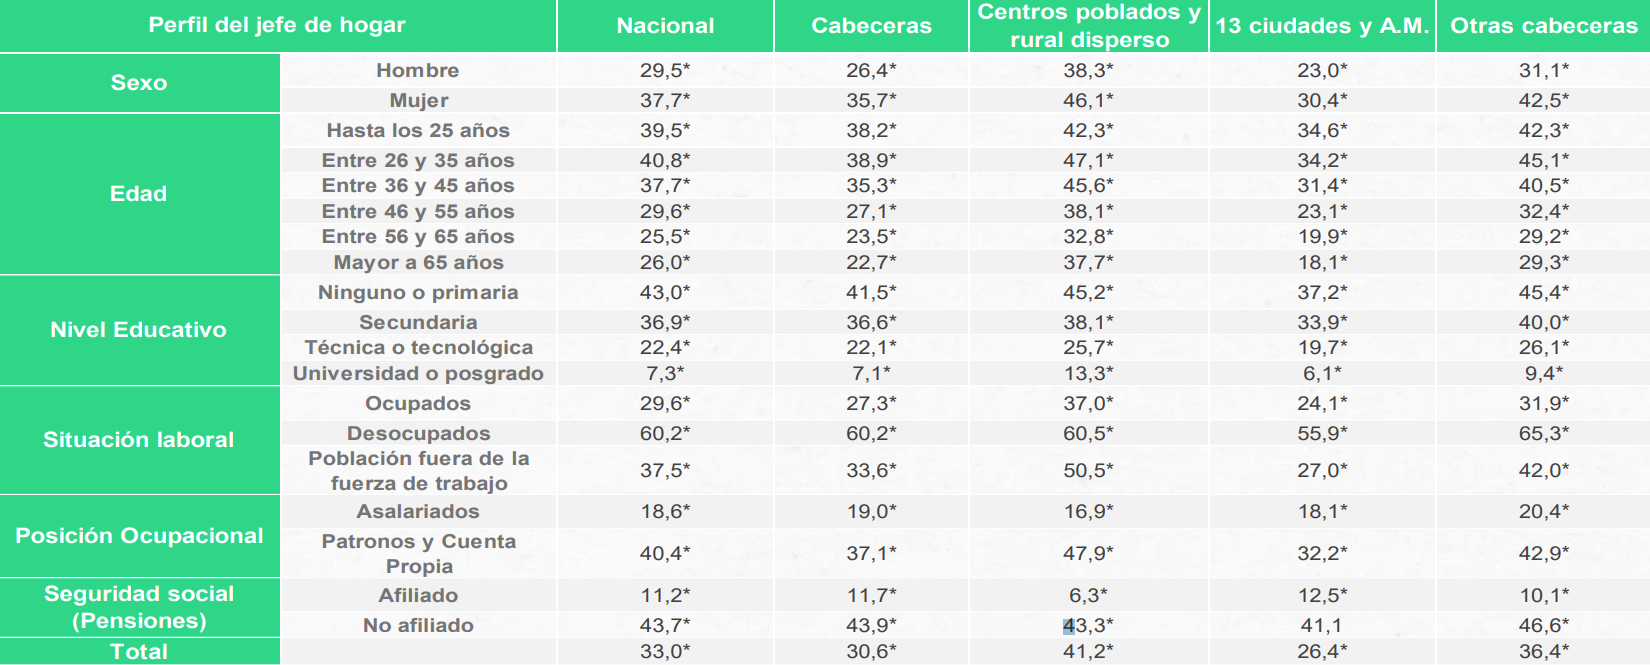
\includegraphics[width=15cm]{img/metodologia/pobrezaMonetariaColombia.png}
        \caption{Incidencias de pobreza monetaria seg\'un perfil del jefe de hogar (porcentaje)}
        \label{fig:pobrezaMonetaria}
    \end{figure}

\begin{itemize}
    \item Edad: 18 - 45 a\~nos
    \item Nivel educativo: Ninguno o primaria
    \item Idioma nativo: Espa\~nol
    \item Intenci\'on: tener una opci\'on de dieta de costo m\'inimo que se adapte a sus necesidades cal\'oricas o nutricionales.
\end{itemize}


\newpage
\subsection{Diagrama de casos de uso}

\noindent Con base en los requerimientos anteriores, se plantea el diagrama de casos de uso en la figura \ref{fig:casosDiagrama}, en el cual se observan los diferentes casos de uso y como se extienden o incluyen otros casos de uso. Como se puede observar en el diagrama, los casos de uso para el usuario se centran en interactuar con el sistema para adaptar la dieta a sus caracter\'isticas y restricciones, y visualizar la dieta.


\begin{figure}[H]
        \centering
        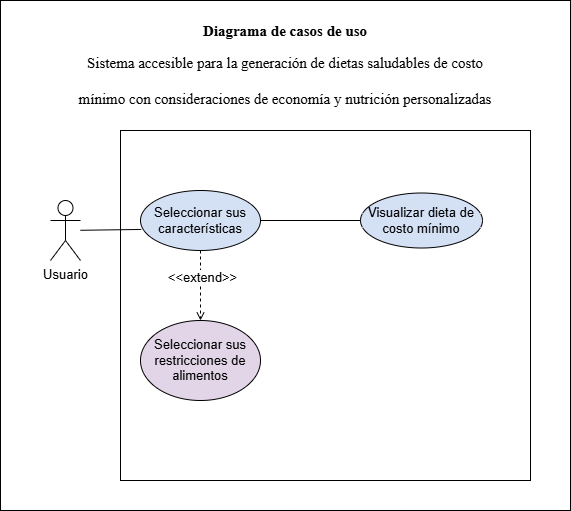
\includegraphics[height=15cm]{img/Diseno/casos de uso.png}
        \caption{Diagrama de casos de uso}
        \label{fig:casosDiagrama}
    \end{figure}



\subsection{Decisiones de tecnolog\'ias}
\noindent Al ser este un proyecto de ingenier\'ia, las tecnolog\'ias que har\'an parte del proyecto son uno de los factores centrales para el desarrollo de este. Por lo que se debe tener claridad   desde el principio de cuales tecnolog\'ias conformar\'an este sistema.

\subsubsection{R}

\noindent Como base de este proyecto, se encuentra el proyecto Foodprice, desarrollado por la Pontificia Universidad Javeriana Cali en colaboraci\'on con Alliance Bioversity \& CIAT; el cual es un paquete en R, el cual es un entorno y lenguaje de programaci\'on con un enfoque matem\'atico\cite{ProjectStatisticalComputing}.

\begin{figure}[H]
        \centering
        
\includegraphics[width=7cm]{img/metodologia/R_logo.svg.png}
        \caption{R logo}
        \label{fig:logoR}
    \end{figure}

Este paquete permite a trav\'es de un modelo matem\'atico calcular dietas de costo m\'inimo en base a algunos par\'ametros y restricciones que elija el usuario; sin embargo, este paquete cuenta con muchos inconvenientes para su uso. Principalmente, R no es un lenguaje amigable para el p\'ublico general, siendo considerado un lenguaje duro de aprender y masterizar\cite{HowLongDoes}. Sumado a esto, el paquete Foodprice no est\'a desarrollado siguiendo las mejores pr\'acticas y est\'andares de programaci\'on, por lo que su modificaci\'on y uso puede llegar a complicarse a\'un m\'as. Agregando adem\'as el hecho de que R es apenas el 21 lenguaje m\'as usado por programadores a nivel mundial, con solo un 4.3\% \cite{MostUsedLanguages}, termina siendo este un lenguaje que a pesar de su poder para c\'alculos estad\'isticos y ciencia de datos, dificulta mucho su uso generalizado; y sobre todo practicamente imposibilita el uso por la poblaci\'on a la que quiere impactar, siendo esta personas en situacion de pobreza, que probablemente no cuenten con los conocimientos y habilidades para poder utilizar un software de estas caracter\'isticas de forma correcta y clara.
\\
\\
\begin{figure}[H]
        \centering
        
\includegraphics[width=7cm]{img/metodologia/Logotipo.png}
        \caption{logo proyecto Foodprice}
        \label{fig:logoFoodprice}
    \end{figure}

Por todos estos motivos, se decide entonces que un factor base para este proyecto es crear un middleware que permita una conexi\'on m\'as sencilla y natural con el paquete de Foodprice, adem\'as de estar construido en una tecnolog\'ia m\'as popular, para as\'i facilitar la posibilidad de que otras entidades o personas puedan consumir o expandir el proyecto Foodprice, llegando as\'i a m\'as personas, potencialmente mejorando la calidad de vida de personas que requieran de una dieta de costo m\'inimo que se adapte a sus necesidades. Adem\'as de esto, se presenta la necesidad de utilizar el paquete Foodprice como una API para poder comunicarse de forma sencilla con python, para lo cual se usar\'a Plumber.

\subsubsection{Plumber}
\noindent Debido a la complejidad de trabajar directamente c\'odigo de R en python, y que las opciones que existen pueden presentar complejidades, sobre todo al trabajar en windows, se opt\'o por usar Plumber para transformar el paquete Foodprice en una API, la cual se consumir\'a mutuamente con otra API de Python, para as\'i comunicarse en lo que se necesite, e invocar las funcionalidades de R desde Python, a  trav\'es de su API. 

\begin{figure}[H]
        \centering
        
\includegraphics[width=7cm]{img/metodologia/plumber.jpeg}
        \caption{logo plumber}
        \label{fig:logoPlumber}
    \end{figure}

Como se mencion\'o anteriormente, Plumber es un paquete en R que permite crear una web API con solamente decorar el codigo de R que ya se tiene, permitiendo as\'i una f\'acil conexi\'on que no requiere de modificar fuertemente el programa ya creado\cite{APIGenerator}.


\subsubsection{Python}
\noindent Como respuesta a lo mencionado anteriormente, se propone Python como lenguaje para el desarrollo del middleware que usar\'a a Foodprice. Esta decisi\'on se toma debido a varios factores, entre los principales la popularidad y el extenso uso que tiene Python en la comunidad de desarrolladores, siendo el tercer lenguaje m\'as usado en 2024 a nivel mundial, con un 51\% de uso\cite{MostUsedLanguages}. Estos factores abrir\'an las puertas al uso del paquete Foodprice para muchos desarrolladores, en conjunto con el middleware en Python.
\begin{figure}[H]
        \centering
        
\includegraphics[width=7cm]{img/metodologia/Python-logo-notext.svg.png}
        \caption{logo Python}
        \label{fig:logoPython}
    \end{figure}

Adem\'as de esto, Python permite una conexi\'on m\'as sencilla y eficiente con aplicaciones web, por lo que es ideal para el prop\'osito de este proyecto.

\subsection{FastAPI}
Para conectar Python como una web API, se hace uso de FastAPI, un web framework r\'apido y moderno, el cual permite crear Apis con Python centr\'andose en la velocidad de rendimiento, y velocidad de codificaci\'on al no ser compleja de usar\cite{FastAPI}.

\begin{figure}[H]
        \centering
        
\includegraphics[width=7cm]{img/metodologia/fastapi.png}
        \caption{logo FastAPI}
        \label{fig:logoFastAPI}
    \end{figure}

Al desarrollar ya ambas APIs, estas se conectar\'an entre si, para comunicarse, y pasar la informaci\'on que se requiera, siendo la aplicaci\'on de Python la que consuma realmente a la de Foodprice en R, y despu\'es de eso se encargue de pasarle la respectiva informaci\'on al front-end para visualizar todo en la aplicaci\'on web.


\subsubsection{ZOD}
\noindent Zod es una biblioteca de validaci\'on y an\'alisis de esquemas de datos dise\~{n}ada para aplicaciones de JavaScript y TypeScript\cite{TypeScriptfirstSchemaValidation}. Se utiliza en este proyecto para encargarse de facilitar la definici\'on, validaci\'on y transformaci\'on de datos de manera estricta y segura.

\begin{figure}[H]
        \centering
        
\includegraphics[width=7cm]{img/metodologia/zod logo.jpg}
        \caption{logo Zod}
        \label{fig:logoZod}
    \end{figure}

\subsubsection{Next.js}
\noindent Next.js es un framework flexible de React que te ofrece bloques de construcci\'on para crear aplicaciones web r\'apidas y completas\cite{ReactFoundationsReact}. Este ser\'a el framework que se utilice en la parte de la construcci\'on de la aplicaci\'on web, siendo este el en cargado del front-end, conect\'andose con el back-end que ser\'an Python y Foodprice. Aprovechando la capacidad de Next.js para crear una aplicaci\'on con elementos visuales interesantes, accesible y de uso intuitivo.

\begin{figure}[H]
        \centering
        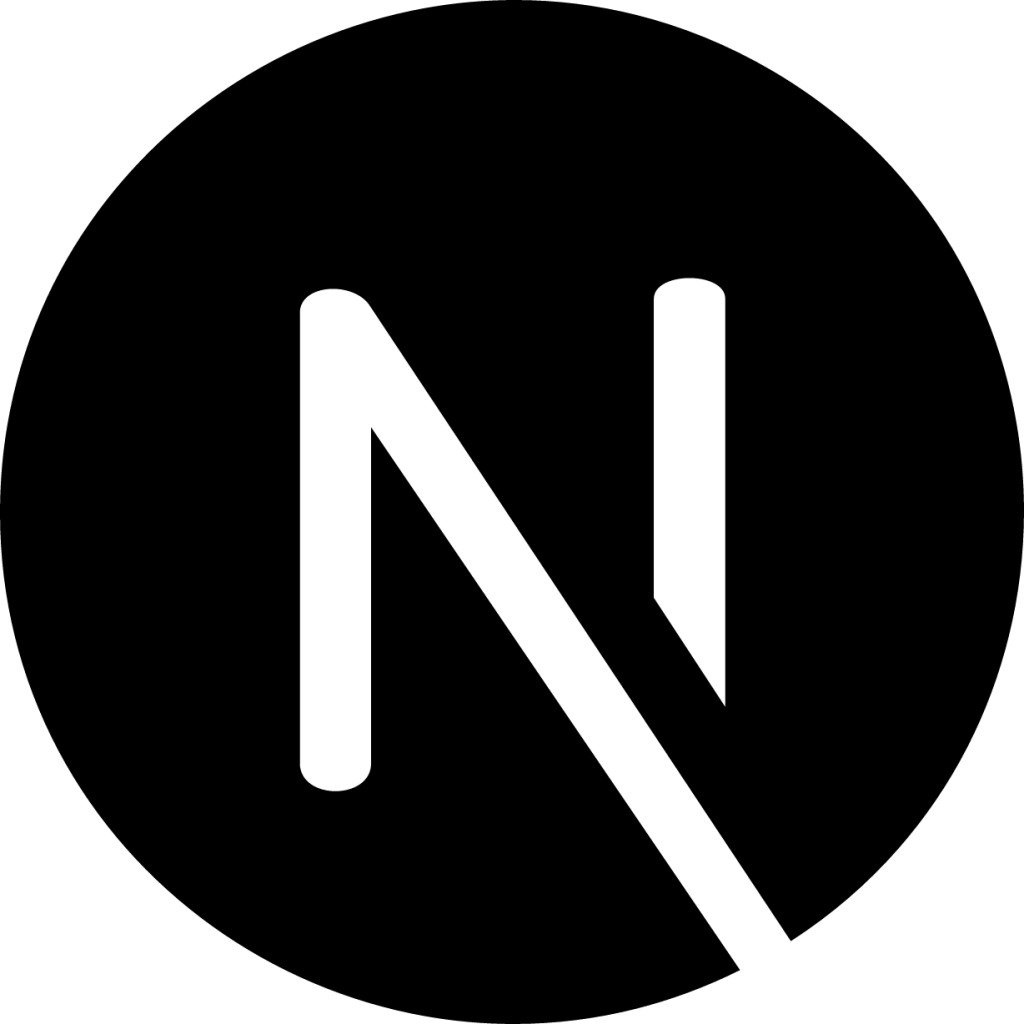
\includegraphics[width=7cm]{img/metodologia/nextjs-icon-1024x1024-5et230l7.png}
        \caption{logo Next.js}
        \label{fig:logoNext}
    \end{figure}

\subsubsection{React}
\noindent React es una biblioteca de JavaScript de c\'odigo abierto desarrollada por Meta (anteriormente Facebook), dise\~{n}ada para construir interfaces de usuario (UI) interactivas y din\'amicas de forma eficiente\cite{React}. Al ser Next.js un framework de React, se utiliza este para el proyecto, aprovechando su facilidad para trabajar de forma modular con componentes para crear as\'i una buena interfaz de usuario.

\begin{figure}[H]
        \centering
        
\includegraphics[width=7cm]{img/metodologia/React-icon.svg.png}
        \caption{logo React}
        \label{fig:logoReact}
    \end{figure}

\subsubsection{React hook form}
\noindent React Hook Form es una biblioteca ligera y eficiente para manejar formularios en aplicaciones React. Est\'a dise\~{n}ada para simplificar la validaci\'on y el manejo de datos de los formularios, aprovechando las caracter\'isticas de los React Hooks para optimizar el rendimiento y proporcionar una experiencia de desarrollo m\'as fluida\cite{ReactHookForm}.


\begin{figure}[H]
        \centering
        
\includegraphics[width=7cm]{img/metodologia/react-hook-form-logo-only.png}
        \caption{logo React hook form}
        \label{fig:logoReactHookForm}
    \end{figure}
    
\subsubsection{Selenium}
\noindent Para conseguir la informaci\'on de los alimentos que representen la realidad de lo que se ve en un supermercado de Cali, se lleg\'o a la conclusi\'on que se requiere de hacer web scraping, ya que estos datos no tienen una API p\'ublica para poder consumirlos. A pesar de que el web scraping es una pr\'actica moralmente ambig\"ua, los datos que se conseguir\'an en este proyecto no se utilizar\'an para generar ninguna ganancia monetaria, y por el contrario se usar\'an para crear un bien para la sociedad. Por lo que con base en que no hay una legislaci\'on clara al respecto, y lo que en casos generales se considera un buen uso de esta t\'ecnica que no tiene problemas legales \cite{juristasRiesgosLegalesWeb2023}, el uso en este proyecto no deber\'ia presentar alg\'un problema. 


\begin{figure}[H]
        \centering
        
\includegraphics[width=7cm]{img/metodologia/Selenium_Logo.png}
        \caption{logo Selenium}
        \label{fig:logoSelenium}
    \end{figure}

Con esto claro, se utilizar\'a Selenium como herramienta de automatizaci\'on con la que se obtendr\'an los datos. Todos los datos que se obtienen a trav\'es de Selenium para este proyecto son p\'ublicos, solo se est\'an extrayendo, y agrupando en una estructura definida, automatizando la b\'usqueda en el portal web de Almacenes \'Exito, y tomando la informaci\'on relevante para este proyecto del producto espec\'ifico.

\subsubsection{Dataframe}
\noindent El dataframe no es exactamente una tecnolog\'ia en s\'i, pero es la manera en la que los datos que son scrapeados con Selenium ser\'an guardados. Con el fin de poder acceder a ellos en cualquier momento desde el paquete en R.

\subsubsection{MongoDB}
\noindent Debido a que no se pueden  realizar queries eficientes al dataframe por ID, se decidi\'o entonces que era necesario tener tambi\'en una base de datos, para permitirle al programa en Python traer de forma eficiente toda la informaci\'on relacionada con cada alimento, y a que el paquete en R no entrega directamente un solo resultado con la dieta exacta requerida, sino varios resultados que cumplen con las restricciones y tipo de dieta, y se debe seleccionar la correcta en Python.

\begin{figure}[H]
        \centering
        
\includegraphics[width=7cm]{img/metodologia/MongoDB_Logo.svg.png}
        \caption{logo MongoDB}
        \label{fig:logoMongoDB}
    \end{figure}


\section{Dise\~no}

\noindent En este apartado se presenta el dise\~no de la arquitectura de la aplicaci\'on, el modelo, as\'i como un bosquejo sencillo inicial de la interfaz de la aplicaci\'on. Para esto, se presentan los diagramas realizados para describir el flujo de la aplicaci\'on, desde aspectos como el usuario dentro de la aplicaci\'on,  hasta el funcionamiento de esta.

\subsection{Arquitectura}
\noindent La arquitectura es un eje central en todo proyecto de software. En este caso, debido a  como cada parte del proyecto se integra entre si, este sistema pertence a la \textbf{Arquitectura Modelo - Vista - Controlador}, esto debido a que se cuenta con tres ejes principales:

\begin{itemize}
    \item Paquete Foodprice: desarrollado en R, este cumple el papel de \textbf{modelo}, encarg\'andose de toda la l\'ogica de consultar a la base de datos, hacer los c\'alculos respectivos con base en la informaci\'on que recibi\'o del modelo, y entregarlo al modelo para que sea visualizado despu\'es por la vista.
    
    \item Middleware Python: Aqu\'i se maneja  la interacci\'on entre la vista y el modelo, recibiendo este la informaci\'on de la vista, haciendo peque\~{n}as tareas de transformar datos para que el modelo los reciba correctamente, e invocando al modelo para que se encargue de toda la l\'ogica y consultas a base de datos (en este caso dataframe); de esta forma cumpliendo el rol de \textbf{controlador}. Sin embargo, en este proyecto no se puede considerar un controlador puro, ya que realiza algunas funciones un poco m\'as complejas, como traer datos de la base de datos de MongoDB para poder tener una eficiencia m\'as alta, ya que el dataframe con el que se trabaj\'o en R no permite hacer queries en base a un id, y el proceso de relacionar cada alimento para traer toda su informaci\'on ser\'ia muy lento. A\'un as\'i se considera que ya que en su mayor\'ia cumple con la tarea de un controlador, que puede aplicarse este rol.

    \item Front-end: El front-end desarrollado en Next.js, el cual se encarga \'unicamente de lo relacionado con la \textbf{vista} y  la interacci\'on con el usuario.
    
\end{itemize}

\begin{figure}[H]
        \centering
        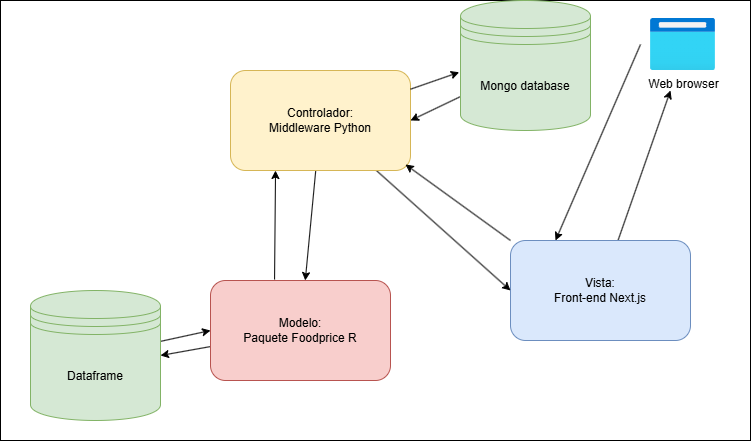
\includegraphics[height=8cm]{img/Diseno/arquitectura.png}
        \caption{Diagrama de la arquitectura del Sistema}
        \label{fig:arquitecturaDiagrama}
\end{figure}

\noindent De esta forma, se observa el diagrama de la arquitectura mencionada anteriormente en la figura \ref{fig:arquitecturaDiagrama}, como el sistema de este proyecto, sigue la arquitectura modelo - vista - controlador, y utiliza el dataframe como una pseudo base de datos, y la base de mongo como una base con informaci\'on m\'as completa sobre cada elemento.

\noindent De la misma manera, al observar la figura \ref{fig:arquitecturaModelo} se puede observar el funcionamiento m\'as detallado del modelo, en el cual le entra la informaci\'on, trae la informaci\'on del dataframe, y realiza los c\'alculos necesarios para devoler una lista de costo m\'inimo de dietas diarias, de las que el controlador debe elegir la relacionada con las caracter\'isticas del usuario.

\begin{figure}[H]
        \centering
        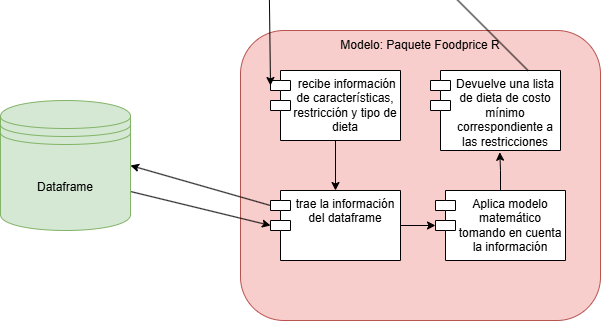
\includegraphics[height=8cm]{img/Diseno/arquitectura modelo.png}
        \caption{Diagrama de la aquitectura - modelo}
        \label{fig:arquitecturaModelo}
    \end{figure}

\noindent As\'i mismo, se cuenta con la arquitectura detallada de la vista en la figura \ref{fig:arquitecturaVista}, aqu\'i se observa  como este elemento  controla toda la interacci\'on con el usuario, siendo aquel que muestra que pantalla se ver\'a dependiendo del estado en el que se encuentre el sistema (se ver\'a m\'as a fondo en el diagrama de flujo en \ref{fig:flujoDiagrama}). Adedm\'as de esto, al interactuar con el usuario, es el que comnienza el proceso de seleccionar las diferentes caracter\'isticas, restricciones, y tipo de dieta. Y al final recibe la dieta correspondiete para mostrarle al usuario.

\begin{figure}[H]
        \centering
        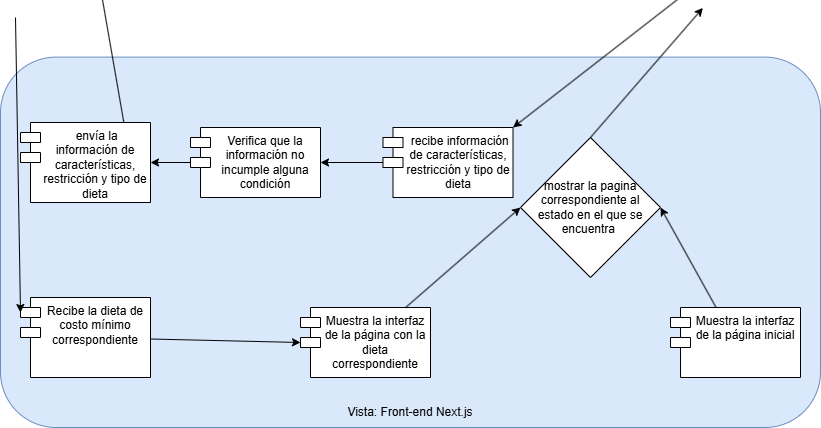
\includegraphics[height=7cm]{img/Diseno/arquitectura vista.png}
        \caption{Diagrama de la aquitectura - vista}
        \label{fig:arquitecturaVista}
    \end{figure}

\noindent En el caso del controlador, en la figura \ref{fig:arquitecturaControlador} se observa como este recibe las entradas de la vista,  las transforma para funcionar de forma correcta con R, y las pasa al modelo; de aqu\'i recibe una lista con dietas de costo m\'inimo, y termina de elegir la correcta, procede a relacionar sus alimentos con el listado completo de la base de Mongo, para entregarle todo eso a la vista de nuevo, y las pueda visualizar.

\begin{figure}[H]
        \centering
        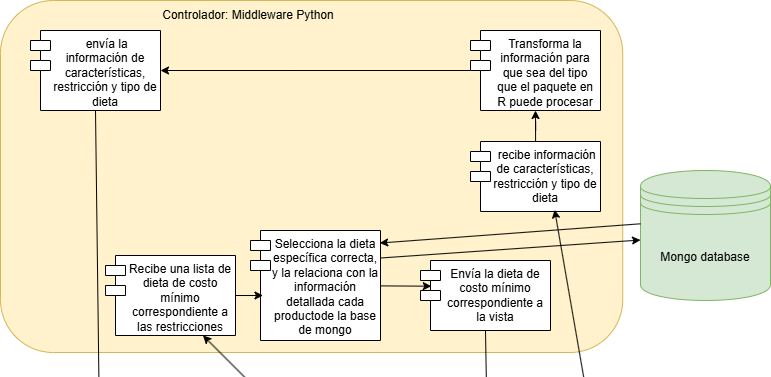
\includegraphics[height=8cm]{img/Diseno/arquitectura controlador.png}
        \caption{Diagrama de la aquitectura - controlador}
        \label{fig:arquitecturaControlador}
    \end{figure}

\noindent Finalmente, como se ve en la figura \ref{fig:arquiCompletaDiagrama} que muestra el diagrama detallada de la arquitectura del prototipo, se toma toda la informaci\'on anterior.

\begin{figure}[H]
        \centering
        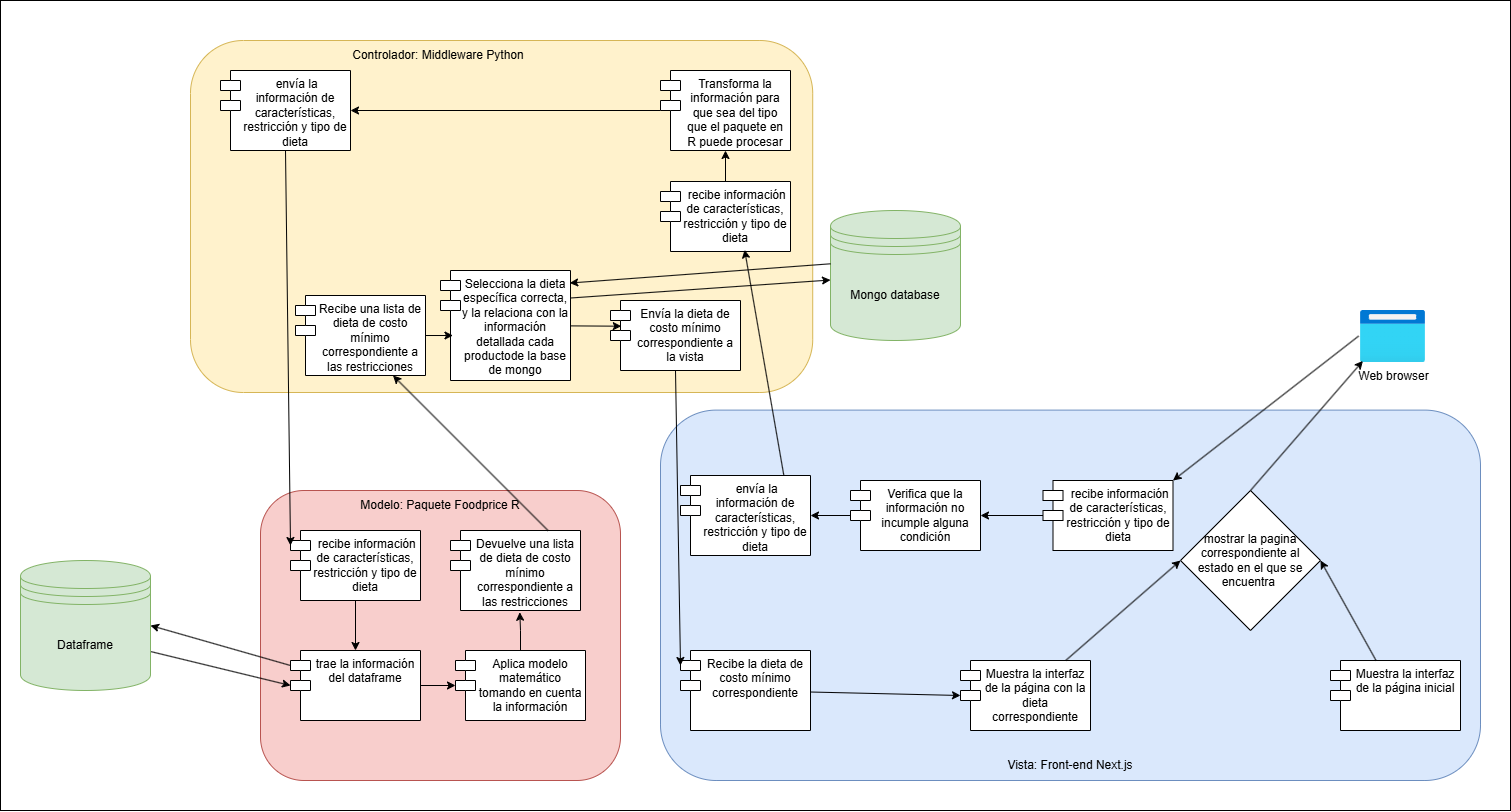
\includegraphics[width=\textwidth]{img/Diseno/arquitectura completa.png}
        \caption{Diagrama de la arquitectura completa detallada}
        \label{fig:arquiCompletaDiagrama}
    \end{figure}

\subsection{Diagrama de flujo}

\noindent En el diagrama de flujo \ref{fig:flujoDiagrama} se observa el flujo del proceso que puede tener el sistema en base a las acciones del usuario y la respuesta de este. Aqu\'i, se contemplan todas los posibles caminos que puede tomar la aplicaci\'on, y se muestran los eventos que llevan a dichos caminos. De esta forma, se empieza con una pantalla inicial, de la cu\'al se pueden seleccionar 3 tipos de opciones a elegir en base a la opci\'on con la que interact\'ue, y as\'i se va navegando en la aplicaci\'on, como se muestra en el diagrama.

\noindent Vale la pena aclarar, que tal al llegar al estado de ver ya la dieta generada, puede decidir volver a la pantalla inicial para generar una nueva sin problema, por lo que el sistema no tiene un estado definitivo de final.
 
 
\begin{figure}[H]
        \centering
        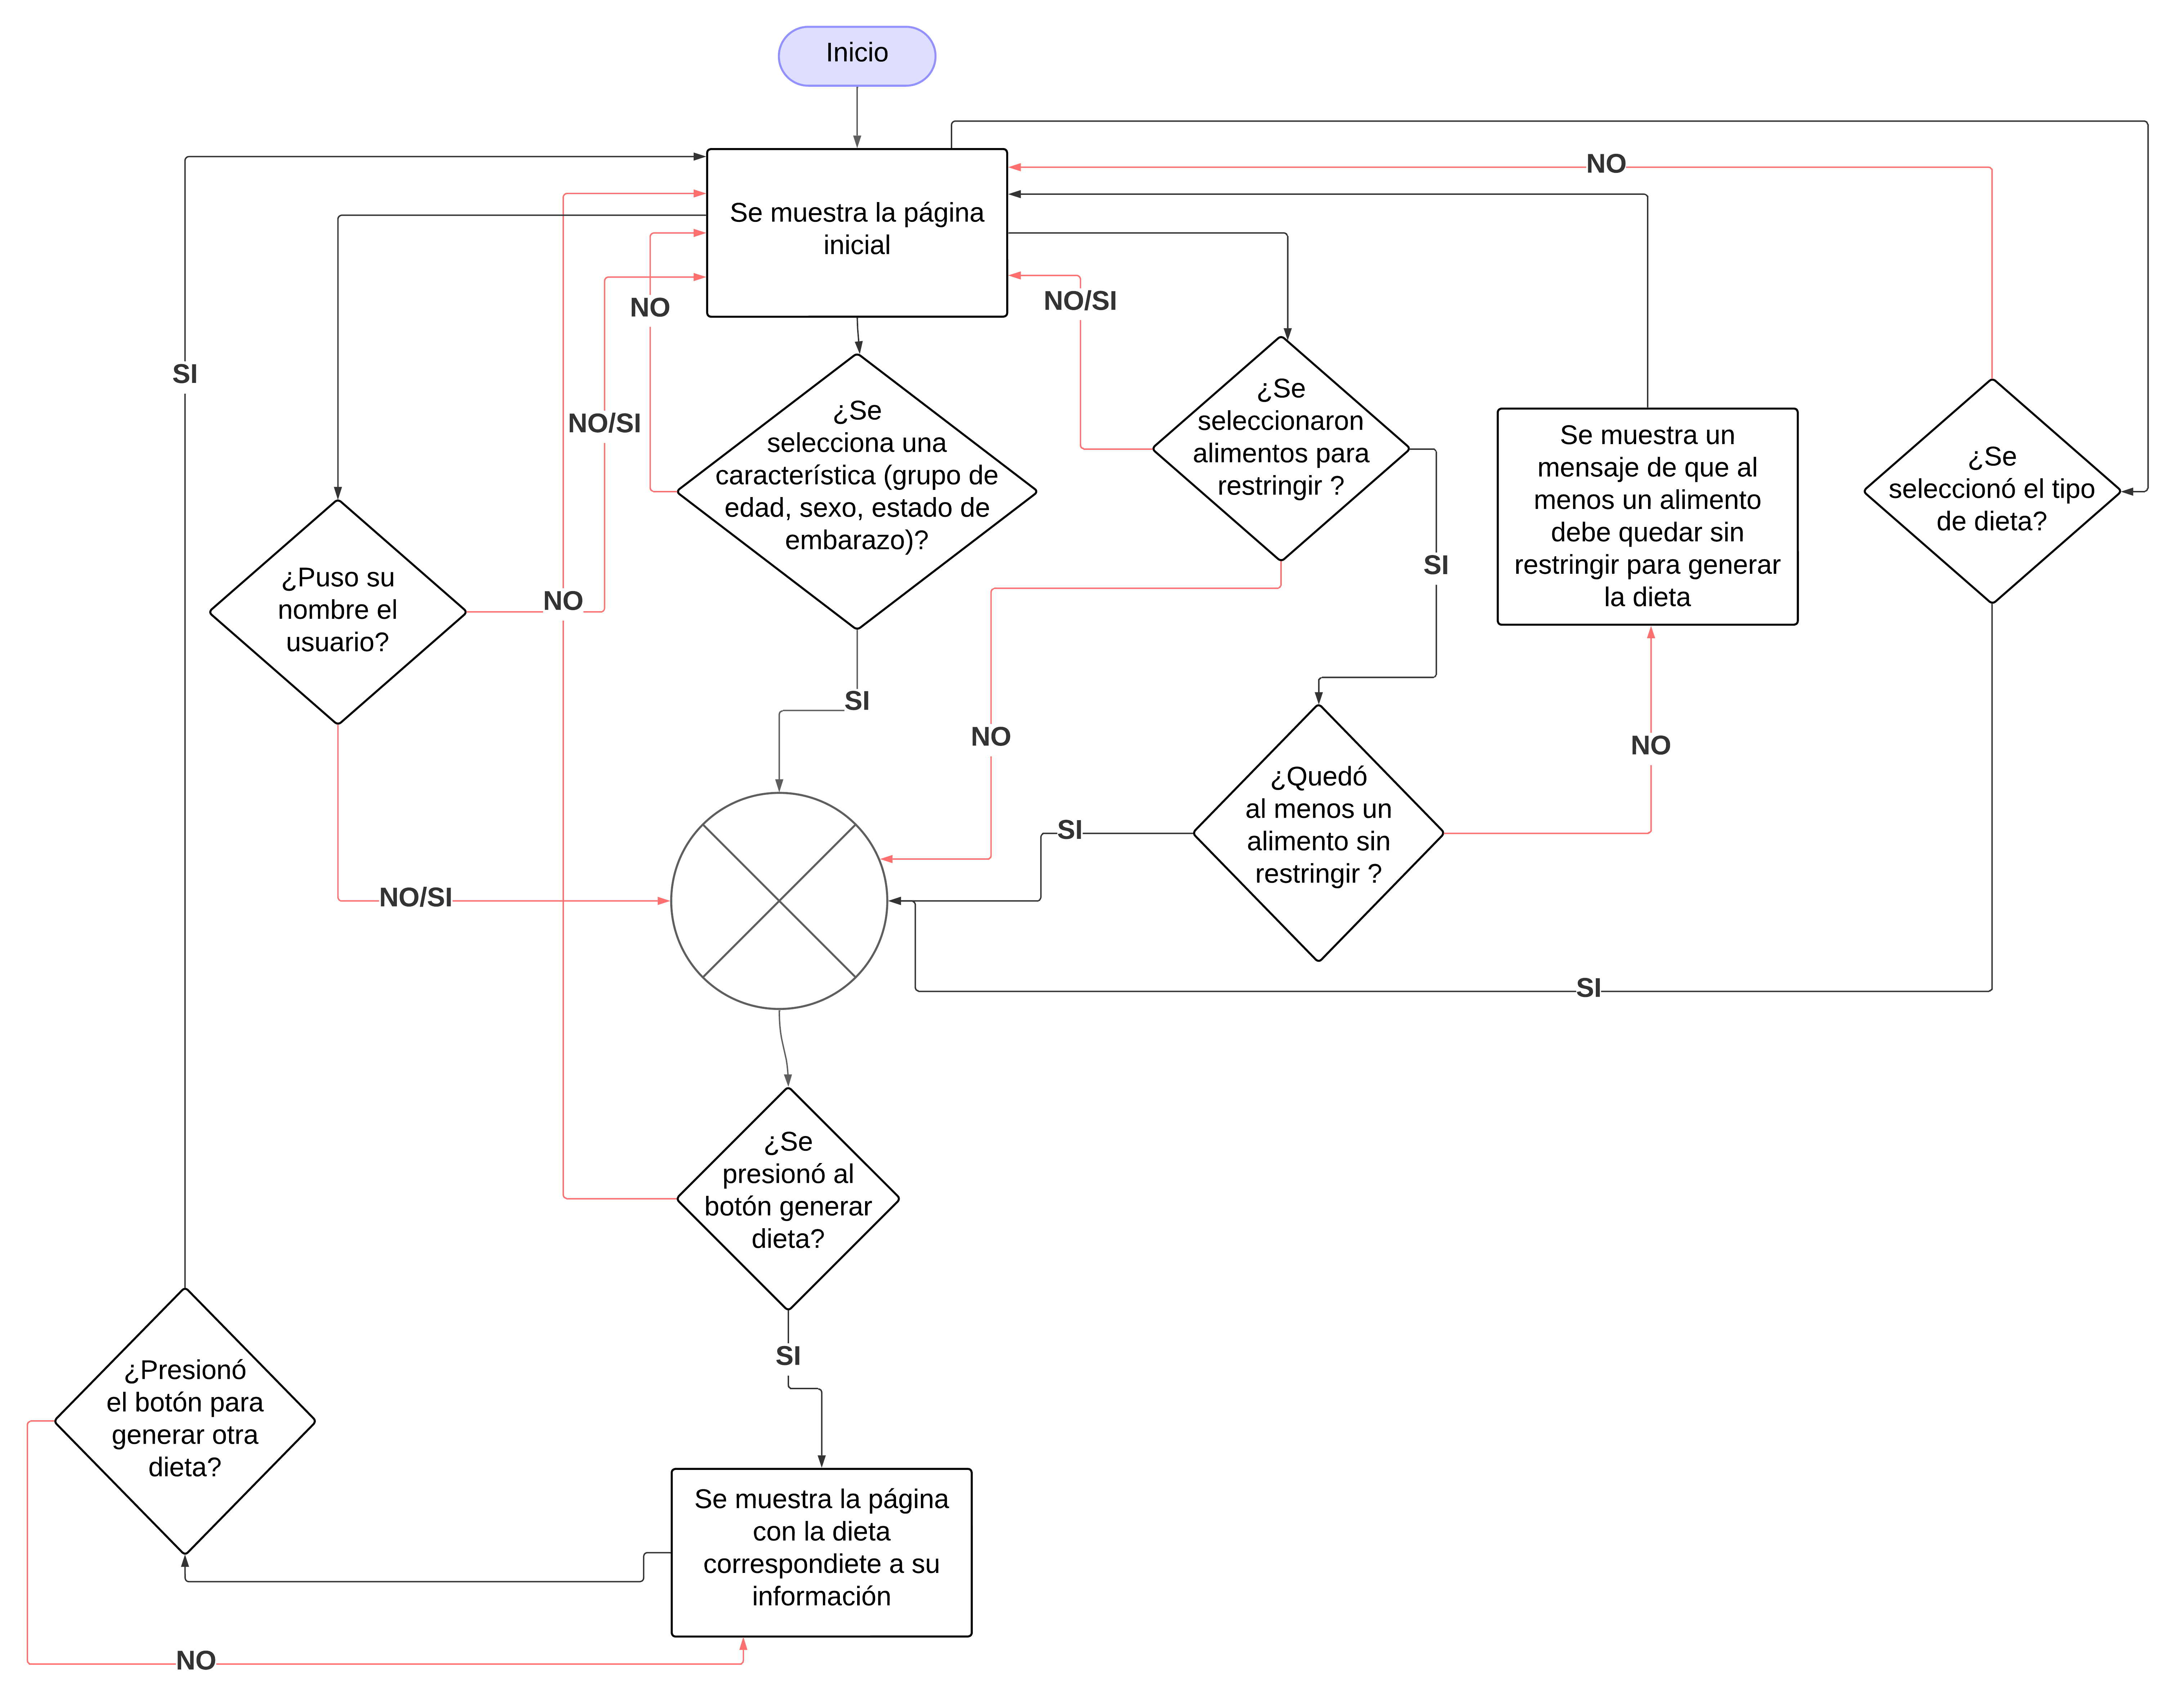
\includegraphics[width=\textwidth]{img/Diseno/flujo.png}
        \caption{Diagrama de flujo del prototipo}
        \label{fig:flujoDiagrama}
    \end{figure}



\subsection{Dise\~no del Modelo de Datos}

\noindent En esta secci\'on se aborda el modelo de datos que se manej\'o para el dise\~no del proyecto, tomando en cuenta que este proyecto consume tanto un paquete en R, como una API en Python, esto present\'o retos a la hora del modelo de datos.
\\
\\
El m\'as grande de estos retos fue el tener que usar dos modelos de datos de naturalezas distintas. Ya que el paquete en R interact\'ua mejor con un dataframe sencillo, del que pueda extraer los datos directamente. Y aunque el programa en  Python  podr\'ia trabajar con este dataframe, esto generar\'ia dificultades debido a queries en base al id que se deben realizar en python, y pueden ser mucho m\'as eficientes al realizarlas sobre una base de datos que permita el uso de ID's. Por este motivo, se decidi\'o entonces tener como parte del sistema tanto un dataframe sencillo para ser consumido por R, como una base de datos m\'as completa en MongoDB para la interacci\'on con Python.
\\
\\
Otro de los grandes retos de este proyecto fue tener que adaptar los datos que se scrapearan del supermercado, para que encajaran con el modelo de datos del paquete en R. Para esto se tuvo que hacer un exhaustivo an\'alisis de como el paquete Foodprice recibe sus datos, para poder adaptarlos.
\\
\\
Sin embargo, los modelos de datos relacionados con el uso directo del paquete en R, terminaron siendo m\'as largas listas que no tenian un orden claro, ya que desde el paquete no se utiliz\'o una estructura clara para los datos, habiendo incluso en ocasiones incongruencias entre los tipos de datos de un mismo campo. Adem\'as de que eran archivos de tipo .RDATA, por lo que no se pod\'ia interactuar con ellos como con una base de datos.
\\
\\
Debido a eso, se presenta aqu\'i en la tabla \ref{tab:modeloDatosAlimentos} el modelo de datos que se usa en la base de datos de MongoDB que se desarroll\'o en este proyecto. Este modelo de datos se asegura de mantener un orden m\'as claro, y sin cambios inesperados. En esta base de datos se guardaron los datos que se consiguieron con el proceso de web scraping, y estos solo se utilizan para interactuar con el sistema a trav\'es de python, relacionando cada alimento con su respectivo alimento en el dataframe que consume el proyecto en R.


\begin{longtable}[c]{| p{.30\textwidth}  | p{.70\textwidth}  |}
    \caption{Modelo de datos de alimentos}
    \label{tab:modeloDatosAlimentos}
    \\ \hline \textbf{Campo} & \textbf{Descripci\'on} \\ \hline
    \endfirsthead
    \hline
    \textbf{Campo} & \textbf{Descripci\'on} \\ \hline
    \endhead
    \hline
    \endfoot
    \hline
    \endlastfoot

    \_id & Identificador \'unico del elemento dentro de MongoDB. \\ \hline
    city & Ciudad de donde proviene el producto. \\ \hline
    store & Tienda de donde proviene el producto. \\ \hline
    name & Nombre del producto. \\ \hline
    url & Enlace hacia el producto. \\ \hline
    price & Precio del producto. \\ \hline
    unit\_price & Precio por cada 100 gramos de producto. \\ \hline
    discount & Descuento con el que cuenta el producto. \\ \hline
    image & Enlace hacia la primera imagen del producto. \\ \hline
    timestamp & Hora a la que fue "scrapeado" el producto. \\ \hline
    TCAC & Identificador del producto dentro de la base de datos de SIPSA (Sistema de Informaci\'on de Precios y Abastecimiento). \\ \hline
    subgroup & Subgrupo de alimentos al que pertenece el producto. \\ \hline

\end{longtable}



\subsection{Dise\~no del prototipo}

\noindent Para el dise\~no del prototipo, se pens\'o en un dise\~no simple e intuitivo, debido al nivel educativo de los usuarios, se decidi\'o que no fuera un sistema complejo de usar, y que tenga textos que ayuden a guiar al usuario a trav\'es de la aplicaci\'on; as\'i como tambi\'en se tom\'o en cuenta que las letras sean legibles y los colores se diferencien f\'acilmente para  as\'i facilitar su uso.
\\
\\
\noindent Tomando en cuenta todos los aspectos anteriores, se cre\'o el prototipo directamente en c\'odigo, pero como un esqueleto sencillo sin funcionalidad real, solamente para tener claros algunos conceptos b\'asicos como el estilo que tendr\'ia la aplicaci\'on, los colores, se defini\'o blanco y negro, y los campos principales.


\begin{figure}[H]
        \centering
        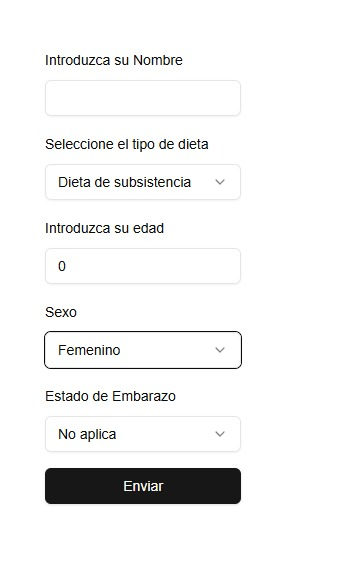
\includegraphics[height=8cm]{img/Diseno/prototipo.png}
        \caption{Prototipo de la aplicaci\'on}
        \label{fig:Prototipo}
    \end{figure}

No se hicieron tantos prototipos de todas las pantallas ya que al hacer un esqueleto sencillo en c\'odigo, se propiciaba el querer avanzar a la siguiente fase para darle funcionalidad final a todo y tomarse su tiempo con cada componente. Por lo que la fase de dise\~{n}o fue m\'as bien corta, pero sirvi\'o de base para en la implementaci\'on tener claro el estilo que se seguir\'ia en la aplicaci\'on en general


\begin{figure}[H]
        \centering
        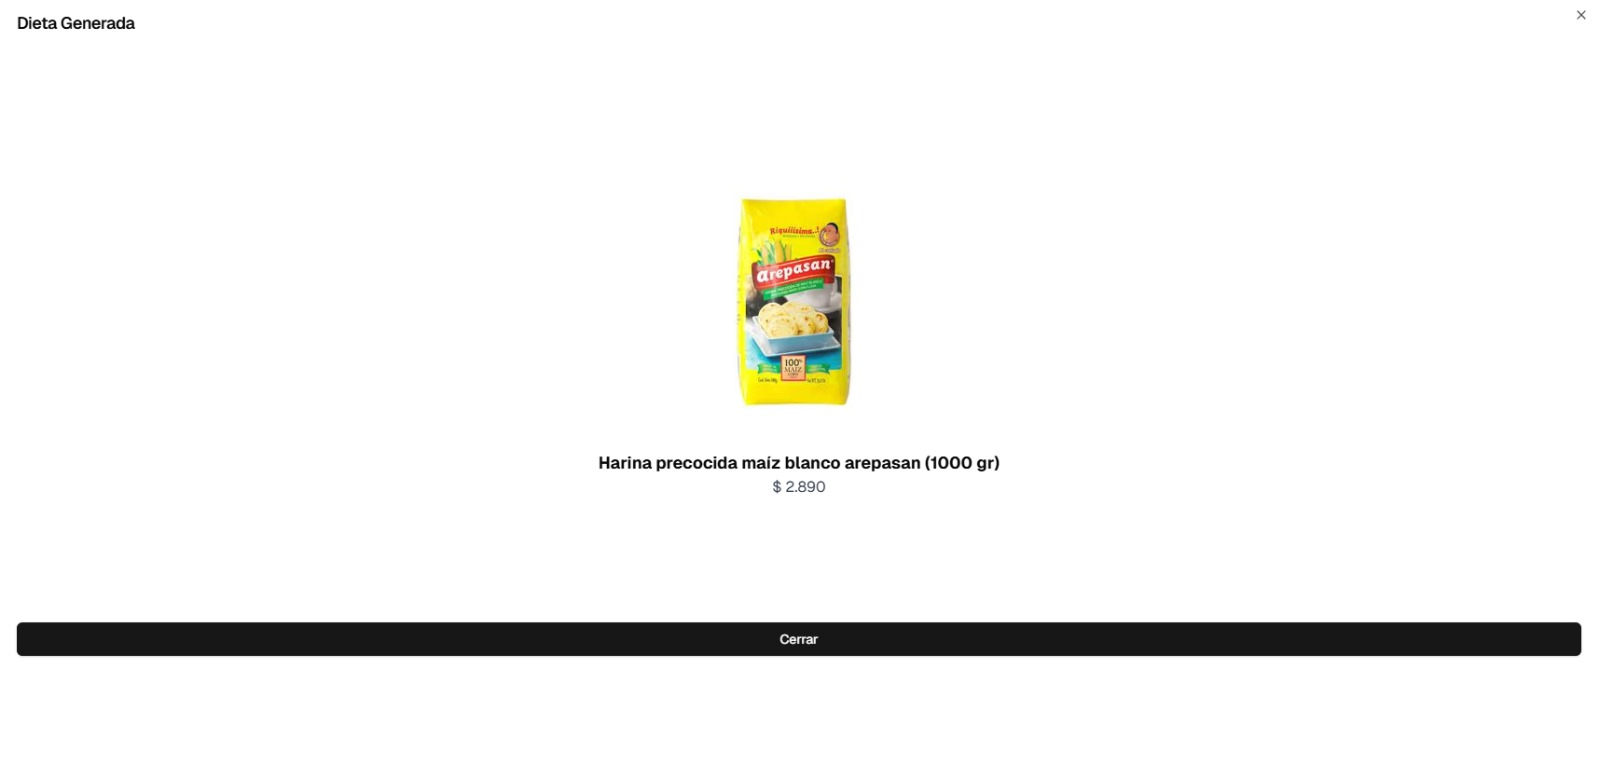
\includegraphics[height=8cm]{img/Diseno/prototipo2.jpeg}
        \caption{Prototipo 2 de la aplicaci\'on}
        \label{fig:Prototipo2}
    \end{figure}

Sin embargo al ver el resultado final de la aplicaci\'on se puede apreciar el avance que hubo desde los prototipos, sobre todo a nivel de facilidad de acceso a la informaci\'on y explicaci\'on de cada elemento, teniendo en cuenta que los usuarios no cuentan con conocimiento previo de la aplicaci\'on.